%!LW recipe=latexmk (lualatex)
%The above command is for use with VSCode as an editor - can be deleted for others

%%%%%%% Instructions %%%%%%%%%%%%%%%%%%%

%Use lualatex to compile with --interaction-mode=nonstopmode
%The commands I run are of the form (in the folder containing thesis.tex): 

%lualatex --aux-directory=./LatexAux --synctex=1 --interaction=nonstopmode --c-style-errors .\thesis.tex
%biber thesis --output-directory=.\LatexAux  

%biber's output-directory should match lualatex's aux-directory or both should be omitted. c-style-errors is optional.
%You can also use latexmk if desired. Beware, sometimes if you have just added alot or are starting fresh,
%it can take more than 5 runs (latexmk's default max) for everything to settle.


% With unicode with lualatex (recommended), do not use amssymb, input/output enc
% Get Error ".. \@ doesn't match definition.."? 
% First, make sure you have ran biber and re-ran lualatex
% Then, try deleting *.aux file of file you were messing with. If needed, escalate to deleting all auxillary files.

%%Using Tikz? Externally generate as pdf (with just normal presets/without tagging) and use includegraphics to add alt text


%%% While drafting, the class options no-mathml and/or no-tag-tree can speed up compiling.
% no-tag-tree cannot be used for final submission. mathml accessiblity tagging is not currently required by ISU

%%%%%%%%%%%%%%%%%%%%%%%%%%%%%%%%%%%%%%%%%%%%%%%%%%%%%%%%%%%%%%%%%%%%%%%%%%%%%%%%%%%%%%%%%%%%%%%%%%%%%%%%%%%%%%%%%%%%%%%%%

\DocumentMetadata{
 lang=en,
 testphase={
  phase-III,
  math,
  table,
  title,
  firstaid
  },
 pdfversion=2.0,
 pdfstandard=ua-2,
 pdfstandard=a-4f,
 %uncompress %can be helpful for debugging
}

%Can pass additional options to packages loaded by the class
%with \PassOptionsToPackage{<options>}{<packagename>}
\PassOptionsToPackage{noend}{algpseudocode}


% Template file for a standard thesis
\documentclass[12pt,math-packages,algorithms-packages]{isuthesistagged}
%packages always loaded in cls file: xpatch, fancyhdr, titlesec, setspace, nowidow, caption
%           subcaption, geometry, graphicx
%biblatex and hyperref must also be loaded later in the preamble




%Additional class options:
% math-packages: loads amsmath,amsthm, mathtools, keytheorems, and associated tagging fixes
% algorithms-packages: loads algorithm, algpseudocode, fixes the numbering, also provides \parstate for long, wrapped states
% no-mathml: disables math tagging (not required by Iowa State)
% no-tag-tree: disables a slow part of tagging (must be re-enabled before submission)
% bib-no-break: by default, page breaks in the middle of bibliography entries are discouraged, but may happen for a particularly long entry (4+ lines).
%       With this option, a page break will never happen in the middle of an entry, no matter how long. This is "recommended" by not required
%       by Iowa State.




%For complex tables
\usepackage{multirow}
\usepackage{pdflscape}

%%Provides math presets: 
%    Sets up some common math presets like Theorem, Definition, etc.
%    Easier to edit or exclude than the class file
\usepackage{templatedTheoremTypes}

%%

%Check package documentation for other font options
%For example, the "default" is a Computer Modern clone
\usepackage[libertinus]{fontsetup}

%Instead of font setup, unicode-math has more fine-tuned control
%\usepackage{unicode-math}

% \setmainfont{texgyrepagella}[
% Extension       = .otf,
% UprightFont     = *-regular,
% ItalicFont      = *-italic,
% BoldFont        = *-bold,
% BoldItalicFont  = *-bolditalic 
% ]
% \setmathfont{texgyrepagella-math.otf}


%Natbib compatibility mode activated
%Different styles available - look at biblatex documentation
\usepackage[natbib=true,refsection=chapter,style=authoryear]{biblatex}
\addbibresource{thesisAccessTest.bib}
\setlength{\bibitemsep}{13.2pt}

%Set the author
\newcommand{\theAuthor}{Alice Wonder}
%Set the tite 
\twoLineTitle{This is the title of a thesis
submitted to Iowa State University on the first line.}{
Second line, only the first letter of
the first word and names
are capitalized!}

%%PDF properties automatically set
\author{\theAuthor}
\title{\titleWithLineBreak}
\usepackage[hypertexnames=false,linktocpage=true,pdfauthor={\theAuthor},pdftitle={\titleWithoutBreak},]{hyperref}
\hypersetup{colorlinks=true,linkcolor=blue,citecolor=blue,filecolor=blue,urlcolor=blue,bookmarksnumbered=true,pdfview=FitB,pdfencoding=auto}
\usepackage{bookmark}


%%%%%%%%%%%%%%%%%%%%%

%%%%%%%%%%%%%%%%%%%%%%%%%%%%%%%%%%
%Optional nomenclature package
\usepackage[notintoc,english]{nomencl}


%The command below can be used to get rid of footnote rule(line)
%\renewcommand*\footnoterule{}

%With unicode instead of bm, symbf should be used
%This remaps \bm to prevent problems. There might be slightly different behavior.
\let\bm\symbf
\begin{document}
% Template Titlepage File
% Please choose appropriate options for Master's thesis, Doctoral dissertations, and creative components. Please read the comments to make an informed choice

\vspace*{-2cm}\titlepage
%%%%%%%%%%%%%%%%%%%

\degree{DOCTOR OF PHILOSOPHY}
\major{Mathematics}
%For co-majors use this command instead of major. Separate the co-majors with a semi-colon
%\comajors{Statistics; Computer Science}

\mprof{John Smith}
% If you have co-major professors, use \mprofs for the first, and \cmprofs for the second 
% instead of mprof
%\mprofs{ABC}
%\cmprofs{DEF}

\format{dissertation}%change to thesis or creative component as needed for a master's
\members{Jane Dee \\ Allen Wrench\\ Katniss Everdeen}
\disclaimertitlepage %sets-up title page to add disclaimer at end
\notice %sets-up title page to add the copyright notice at the bottom

%%%%%%
% "A <format> submitted to <the graduate faculty>..." can
% be changed to something other than graduate faculty with
% this command:
% \submit{the graduate faculty alternative}

\maketitle

\frontmattersetup
% %%
% % Optional thesis dedication
%   Dedication is not usually listed in the table of contents.
%   However, if you do want it, add this command here (not in the dedication file)
%   \addToTOCWithoutChapter{DEDICATION}
\include{Preface/dedication}

\tableofcontentsTagged
\cleardoublepage \phantomsection
\pagebreak

\listoftablesTagged %remove if no tables

\cleardoublepage \phantomsection
\listoffiguresTagged %remove if no figures

%Optional nomenclature
%\cleardoublepage \phantomsection
%\nomenclatureTagged

%Adds Chapter in front of chapter on TOC
\addtocontents{toc}{\def\protect\@chapapp{CHAPTER\ }}

%Optional Acknowledgements
\cleardoublepage \phantomsection
\include{Preface/acknowl}
%Required thesis abstract
\cleardoublepage \phantomsection
\include{Preface/abstract}
\newpage
\pagenumbering{arabic}
\pagestyle{fancy}
% Chapter 1 of the Thesis Template File
\chapter{General Introduction}
% Chapter titles are to be all caps and are automatically formatted so.
% If you have an exception and need lower-case letters outside of math (which are automatically ignored),
% you can use \NoCaseChange{....} around what should be protected

This chapter will have the introduction to your thesis as a whole.

This is the opening paragraph to my thesis which
explains in general terms the concepts and hypothesis
which will be explored in my thesis.

With more general information given here than really
necessary.

\section{Overview Two Words}

Here initial concepts and conditions are explained and
several hypothesis are mentioned in brief.

\subsection{Hypothesis}

Here one particular hypothesis is explained in depth
and is examined in the light of current literature.

\subsubsection{Parts of the hypothesis}

Here one particular part of the hypothesis that is
currently being explained is examined and particular
elements of that part are given careful scrutiny.

% % Below \subsubsection
% % Sectional commands: \paragraph and \subparagraph may also be used

\subsection{Second Hypothesis}

Here one particular hypothesis is explained in depth
and is examined in the light of current literature.

\subsubsection{Parts of the second hypothesis}

Here one particular part of the hypothesis that is
currently being explained is examined and particular
elements of that part are given careful scrutiny
\autocite{buiEveryGeneratingPolytope2023}, abcd.

\section{Criteria Review}

Here certain criteria are explained thus eventually
leading to a foregone conclusion.
\begin{theorem}
    Here's a theorem!
\end{theorem}

\printbibliography[heading=subbibnumbered]

\chapter{Paper 1 Title Goes Here}
\label{polymer_fibers}
% Chapter titles are to be all caps and are automatically formatted so.
% If you have an exception and need lower-case letters outside of math (which are automatically ignored),
% you can use \NoCaseChange{....} around what should be protected

\begin{center}
    Authors and Affiliations \\
    %The changes suggest this is supposed to be a footnote ... so we are just guessing over here
    Modified from a manuscript to be submitted to/ under review/ published in \textit{Name of the Journal}
    \blfootnote{A version of this chapter appears in Journal of Discipline, Volume 18, Issue 3}
\end{center}

\section{Abstract}
This is the text of my abstract that is part of the thesis itself.
The abstract describes the work in the first paper general. You can use the same abstract as your paper here.

%\pagebreak %remove if needed

% Please include sections as the paper has, some of the following sections are meant as examples of what can be done, the bibliography should be made as given

\section{Overview}

The  construct of this section or any further section is same as the authors paper.
This is the opening paragraph to my thesis which
explains in general terms the concepts and hypothesis
which will be used in my thesis.

With more general information given here than really
necessary.

\section{Introduction}

Here initial concepts and conditions are explained and
several hypothesis are mentioned in brief.

\autocite{kleeHellyTheoremIts1963} the definitive model is seen.

\subsection{Hypothesis}

Here one particular hypothesis is explained in depth
and is examined in the light of current literature.

\subsubsection{Parts of the hypothesis}

Here one particular part of the hypothesis that is
currently being explained is examined and particular
elements of that part are given careful scrutiny.

% Below \subsubsection
% Sectional commands: \paragraph and \subparagraph may also be used

\subsection{Second Hypothesis}

\paragraph{Heading} Here one particular hypothesis is explained in depth
and is examined in the light of current literature. \subparagraph{Even smaller heading} Another sentence.

\subsubsection{Parts of the second hypothesis}

Here one particular part of the hypothesis that is
currently being explained is examined and particular
elements of that part are given careful scrutiny.
\begin{theorem}
    If true, then this theorem is vacuous.
\end{theorem}

\section{Criteria Review}

Here certain criteria are explained thus eventually
leading to a foregone conclusion.

\section{Conclusion}\label{conclusion}

The conclusion of the paper goes here.
%%%%%%%%
\autocite{buiEveryGeneratingPolytope2023}
%%%%
% Reference section comes before the appendix

\printbibliography[heading=subbibnumbered]

%%%%%
%% Appendix
% This section may or may not be included
% Chapter 2 shows a double appendix example. Please use A or B as in Appendix A if there are multiple appendix. Use "Appendix A:" before writing the title
% Chapter 3 shows a single appendix example. Use "Appendix:" before writing the title 
\section{Appendix A: Appendix A Title Goes Here After The Colon}
If there is an appendix that needs to go with the paper it can be as a section \autocite{kleeHellyTheoremIts1963}

\subsection{Procedure details}
Details of the paper specific appendix procedures

% This section may or may not be included

\section{Appendix B: Appendix B Title Goes Here After The Colon}
If there is an appendix that needs to go with the paper it can be as a section \autocite{chenGraphHomotopyGraham2001}

\subsection{Procedure details}
Details of the paper specific appendix procedures
\chapter{Paper 2 Title Goes Here}
% Chapter titles are to be all caps and are automatically formatted so.
% If you have an exception and need lower-case letters outside of math (which are automatically ignored),
% you can use \NoCaseChange{....} around what should be protected

\begin{center}
    Authors and Affiliations \\
    Modified from a manuscript to be submitted to/ under review/ published in \textit{Name of the Journal}
    \blfootnote{A version of this chapter appears in Journal of Discipline, Volume 18, Issue 3}
\end{center}

\section{Abstract}
This is the text of my abstract that is part of the thesis itself.
The abstract describes the work in the first paper general. You can use the same abstract as your paper here.

%\pagebreak %remove if needed

% Please include sections as the paper has, some of the following sections are meant as examples of what can be done, the bibliography should be made as given

\section{Overview}

The  construct of this section or any further section is same as the authors paper.
This is the opening paragraph to my thesis which
explains in general terms the concepts and hypothesis
which will be used in my thesis.

With more general information given here than really
necessary.
\begin{figure}[b]
    \centering
    \begin{subfigure}[c]{0.495\textwidth}
        \includegraphics[alt={sample image},width=0.99\textwidth]{example-image-c}%
        \subcaption{\label{fig:2a}}
    \end{subfigure}
    \begin{subfigure}[c]{0.495\textwidth}
        \centering{\includegraphics[alt={sample image},width=0.99\textwidth]{example-image-c}}%
        \subcaption{\label{fig:2b}}%
    \end{subfigure}%
    \caption{A figure with two subfigures: (a) first subfigure; (b) second subfigure.\label{fig:2}}
\end{figure}

\section{Introduction}

Here initial concepts and conditions are explained and
several hypothesis are mentioned in brief.

did the initial work
the definitive model is seen.

\subsection{Hypothesis}

Here one particular hypothesis is explained in depth
and is examined in the light of current literature.

\subsubsection{Parts of the hypothesis}

Here one particular part of the hypothesis that is
currently being explained is examined and particular
elements of that part are given careful scrutiny.

% Below \subsubsection
% Sectional commands: \paragraph and \subparagraph may also be used

\subsection{Second Hypothesis}

Here one particular hypothesis is explained in depth
and is examined in the light of current literature.

\subsubsection{Parts of the second hypothesis}

Here one particular part of the hypothesis that is
currently being explained is examined and particular
elements of that part are given careful scrutiny.

\addtocontents{toc}{\protect\newpage} %% Remove this if needed, this lines forces the lines of the TOC starting with the below sub-heading "Critical Review" to go to the next page. Remove this formatting line as it will be required only if you want to force a table of contents entry to the next page along with the other subsequent entries.

\section{Criteria Review}

Here certain criteria are explained thus eventually
leading to a foregone conclusion.

\section{Conclusion}\label{Conclusion1}

The conclusion of the paper goes here.

\autocite{zieglerLecturesPolytopes1995}
\autocite{superLong}
%%%%
% Reference section comes before the appendix

\printbibliography[heading=subbibnumbered]

%%%%%
%% Appendix
% This section may or may not be included
% Chapter 2 shows a double appendix example. Please use A or B as in Appendix A if there are multiple appendix. Use "Appendix A:" before writing the title
% Chapter 3 shows a single appendix example. Use "Appendix:" before writing the title 
\section{Appendix: Appendix Title Goes Here}
If there is an appendix that needs to go with the

\subsection{Procedure details}
Details of the paper specific appendix procedures

\part{Let us have a part page}
\chapter{\MakeUppercase{Paper 3 Title Goes Here}}
% \MakeUppercase{} is conveninent, but if it causes undesired
%behavior (perhaps due to acronyms or math), you can just manually capitalize your chapter title
% \chaper{GENERAL INTRODUCTION}

\begin{center}
    Authors and Affiliations \\
    Modified from a manuscript to be submitted to/ under review/ published in \textit{Name of the Journal}
    \blfootnote{A version of this chapter appears in Journal of Discipline, Volume 18, Issue 3}
\end{center}

\section{Abstract}
This is the text of my abstract that is part of the thesis itself.
The abstract describes the work in the first paper general. You can use the same abstract as your paper here.
I want to also refer you to \autoref{methods} for more about the procedures.
%\pagebreak %remove if needed

% Please include sections as the paper has, some of the following sections are meant as examples of what can be done, the bibliography should be made as given

\section{Methods and procedures}
\label{methods}

This is the opening paragraph to my thesis which
explains in general terms the concepts and hypothesis
which will be used in my thesis.

With more general information given here than really
necessary.

\section{Introduction}

Here initial concepts and conditions are explained and
several hypothesis are mentioned in brief.

As can be seen in \autoref{nothing} it is truly
obvious what I am saying is true.

\begin{table}[h!tb] \centering
    \caption[This table shows a standard non-empty table. Please check the code caption for extended instructions]{This table shows a standard empty table. In case of long captions, we want to use the long caption as the description to the table and image but not use it in the table of contents and list of figures/ tables. In order to do this, there are two captions which have been provided, remove the first square bracket options if there is only one small caption. You can use citations like this to}
    %use \tagpdfsetup{table/tagging=presentation} if and only if the table
    %is for alignment/presentation purposes and is not a real table
    %
    %\tagpdfsetup{table/header-rows={1,2}} would have rows 1 and 2 be header rows
    \tagpdfsetup{table/header-rows={1}}
    %Use \tagpdfsetup{table/header-columns={}} for header columns instead
    %Put \tagpdfsetup{table/multirow={⟨number of rows⟩}} in cells spanning multiple rows
    %Note, multicolumn works automatically (no extra commands necessary)

    \begin{tabular}{ll}
        Bach      & Cello Suite Number 1  \\
        Beethoven & Cello Sonata Number 3 \\
        Brahms    & Cello Sonata Number 1
    \end{tabular}
    \label{nothing}

    \vspace{ 2 in}
\end{table}

\subsection{Hypothesis}

Here one particular hypothesis is explained in depth
and is examined in the light of current literature.

This can also be seen in \autoref{moon} that the
rest is obvious.

\begin{figure}[h!tb] \centering

    \vspace{ 2 in}
    \caption{This table shows a standard empty figure}
    \label{moon}
\end{figure}

\subsubsection{Parts of the hypothesis}

Here one particular part of the hypothesis that is
currently being explained is examined and particular
elements of that part are given careful scrutiny.

% Below \subsubsection
% Sectional commands: \paragraph and \subparagraph may also be used

\subsection{Second Hypothesis}

Here one particular hypothesis is explained in depth
and is examined in the light of current literature.

\subsubsection{Parts of the second hypothesis}

Here one particular part of the hypothesis that is
currently being explained is examined and particular
elements of that part are given careful scrutiny.

%\addtocontents{toc}{\protect\newpage} % Adds \newpage in "\tableofcontents"
\section{Criteria Review}

Here certain criteria are explained thus eventually
leading to a foregone conclusion as can be seen in
\autoref{nevermore}.

\begin{table}[h!tb] \centering
    \captionsetup{width=2in}
    \caption{This table shows a standard empty table with a limited caption width}
    \label{nevermore}

    \vspace{ 2 in}
\end{table}
\section{Continuing Tables}
Note, tables with cells spanning multiple columns work automatically, but cells spanning multiple rows require extra tagging.
\begin{table}[ht]
    \caption{This is a two-part table doing things.}
    %
    %use \tagpdfsetup{table/tagging=presentation} if and only if the table
    %is for alignment/presentation purposes and is not a real table
    %
    %\tagpdfsetup{table/header-rows={1,2}} would have rows 1 and 2 be header rows
    \tagpdfsetup{table/header-rows={1}}
    %Use \tagpdfsetup{table/header-columns={}} for header columns instead
    %Put \tagpdfsetup{table/multirow={⟨number of rows⟩}} in cells spanning multiple rows
    %Note, multicolumn works automatically (no extra commands necessary)

    \begin{tabular}{rrrlrrrr}
        k      & q          & p+ & p- & s1                                                         & s2                                                         & s3                                                         & RHS       \\ \hline
        2      & 2          & 2  & 1  & 1                                                          & 0                                                          & 0                                                          & 1         \\
        -T     & 0          & 1  & 1  & 0                                                          & 1                                                          & 0                                                          & 0         \\
        T      & -1         & 0  & 1  & 0                                                          & 0                                                          & 1                                                          & 0         \\
        -1     & 1          & -1 & 1  &                                                            &                                                            &                                                            &           \\ \hline
        2(T+1) & 2          & 0  & 1  & 1                                                          & -2                                                         & 0                                                          & 1         \\ \hline
        -T     & 0          & 1  & 1  & 0                                                          & 1                                                          & 0                                                          & 0         \\
        T      & -1         & 0  & 1  & 0                                                          & 0                                                          & 1                                                          & 0         \\
        -(T+1) & 1          & 0  & 1  & 0                                                          & 1                                                          & 0                                                          &           \\ \hline
        0      & 2+2(T+1)/T & 0  & 1  & 1                                                          & -2                                                         & -2(T+1)/T                                                  & 1         \\ \hline
        0      & -1         & 1  & 1  & 0                                                          & 1                                                          & 1                                                          & 0         \\
        1      & -1/T       & 0  & 1  & 0                                                          & 0                                                          & 1/T                                                        & 0         \\
        0      & 1-(T+1)/T  & 0  & 1  & 0                                                          & 1                                                          & (T+1)/T                                                    &           \\ \hline
        0      & 2(2T+1)/T  & 0  & 1  & 1                                                          & -2                                                         & -2(T+1)/T                                                  & 1         \\ \hline
        0      & -1         & 1  & 1  & 0                                                          & 1                                                          & 1                                                          & 0         \\
        1      & -1/T       & 0  & 1  & 0                                                          & 0                                                          & 1/T                                                        & 0         \\
        0      & -1/T       & 0  & 1  & 0                                                          & 1                                                          & (T+1)/T                                                    &           \\ \hline
        0      & 1          & 0  & 1  & T/2(2T+1)                                                  & -T/(2T+1)                                                  & -1                                                         & T/2(2T+1) \\ \hline
        0      & 0          & 1  & 1  & T/2(2T+1)                                                  & 1-T/(2T+1)                                                 & 0                                                          & T/2(2T+1) \\
        1      & 0          & 0  & 1  & 1/2(2T+1)                                                  & -1/(2T+1)                                                  & 0                                                          & 1/2(2T+1) \\ \hline
        0      & 0          & 0  & 1  & 1/2(2T+1)                                                  & 1-1/(2T+1)                                                 & -1+(T+1)/TT                                                &           \\ \hline
        0      & 0          & 0  & 1  & 1/2(2T+1)                                                  & 1-1/(2T+1)                                                 & -1+(T+1)/TT                                                &           \\ \hline
        0      & 0          & 0  & 0  & \tagpdfsetup{table/multirow={8}}\multirow{8}{*}{1/2(2T+1)} & \tagpdfsetup{table/multirow={8}}\multirow{8}{*}{1/2(2T+1)} & \tagpdfsetup{table/multirow={8}}\multirow{8}{*}{1/2(2T+1)} &           \\ \cline{1-4}
        0      & 0          & 0  & 0  &                                                            &                                                            &                                                            &           \\ \cline{1-4}
        0      & 0          & 0  & 0  &                                                            &                                                            &                                                            &           \\ \cline{1-4}
        0      & 0          & 0  & 0  &                                                            &                                                            &                                                            &           \\ \cline{1-4}
        0      & 0          & 0  & 0  &                                                            &                                                            &                                                            &           \\ \cline{1-4}
        0      & 0          & 0  & 0  &                                                            &                                                            &                                                            &           \\ \cline{1-4}
        0      & 0          & 0  & 0  &                                                            &                                                            &                                                            &           \\ \cline{1-4}
        0      & 0          & 0  & 0  &                                                            &                                                            &                                                            &           \\ \hline
    \end{tabular}
\end{table}
\begin{table}[ht]
    %As a continued table, use \ContinuedFloat to keep the same #
    %And use the text "Continued" inside the caption
    \ContinuedFloat
    \caption{Continued}
    %
    %use \tagpdfsetup{table/tagging=presentation} if and only if the table
    %is for alignment/presentation purposes and is not a real table
    %
    %\tagpdfsetup{table/header-rows={1,2}} would have rows 1 and 2 be header rows
    \tagpdfsetup{table/header-rows={1}}
    %Use \tagpdfsetup{table/header-columns={}} for header columns instead
    %Put \tagpdfsetup{table/multirow={⟨number of rows⟩}} in cells spanning multiple rows
    %Note, multicolumn works automatically (no extra commands necessary)

    \begin{tabular}{rrrlrrrr}
        k      & q          & p+ & \multicolumn{1}{r}{p-} & s1        & s2         & s3          & RHS       \\ \hline
        2      & 2          & 2  & \multicolumn{1}{r}{-2} & 1         & 0          & 0           & 1         \\
        -T     & 0          & 1  & -1                     & 0         & 1          & 0           & 0         \\
        T      & -1         & 0  & 0                      & 0         & 0          & 1           & 0         \\
        -1     & 1          & -1 & \multicolumn{1}{r}{1}  &           &            &             &           \\ \hline
        2(T+1) & 2          & 0  & 0                      & 1         & -2         & 0           & 1         \\ \hline
        -T     & 0          & 1  & -1                     & 0         & 1          & 0           & 0         \\
        T      & -1         & 0  & 0                      & 0         & 0          & 1           & 0         \\
        -(T+1) & 1          & 0  & 0                      & 0         & 1          & 0           &           \\ \hline
        0      & 2+2(T+1)/T & 0  & 0                      & 1         & -2         & -2(T+1)/T   & 1         \\ \hline
        0      & -1         & 1  & \multicolumn{1}{r}{-1} & 0         & 1          & 1           & 0         \\
        1      & -1/T       & 0  & 0                      & 0         & 0          & 1/T         & 0         \\
        0      & 1-(T+1)/T  & 0  & 0                      & 0         & 1          & (T+1)/T     &           \\ \hline
        0      & 2(2T+1)/T  & 0  & 0                      & 1         & -2         & -2(T+1)/T   & 1         \\ \hline
        0      & -1         & 1  & \multicolumn{1}{r}{-1} & 0         & 1          & 1           & 0         \\
        1      & -1/T       & 0  & 0                      & 0         & 0          & 1/T         & 0         \\
        0      & -1/T       & 0  & 0                      & 0         & 1          & (T+1)/T     &           \\ \hline
        0      & 1          & 0  & \multicolumn{1}{r}{0}  & T/2(2T+1) & -T/(2T+1)  & -1          & T/2(2T+1) \\ \hline
        0      & 0          & 1  & \multicolumn{1}{r}{-1} & T/2(2T+1) & 1-T/(2T+1) & 0           & T/2(2T+1) \\
        1      & 0          & 0  & \multicolumn{1}{r}{0}  & 1/2(2T+1) & -1/(2T+1)  & 0           & 1/2(2T+1) \\ \hline
        0      & 0          & 0  & 0                      & 1/2(2T+1) & 1-1/(2T+1) & -1+(T+1)/TT &           \\ \hline
    \end{tabular}
\end{table}

\section{Results}
Include any results

\section{Conclusion}\label{conclusion2}

The conclusion of the paper goes here.

%\autocite{allen}, \autocite{bruner} 
\autocite{dochtermannMinimalGraphsContractible2023}
\autocite{superLong}
%%%%
% Reference section comes before the appendix

\printbibliography[heading=subbibnumbered]

%%%%%
%% Appendix
% This section may or may not be included
% Chapter 2 shows a double appendix example. Please use A or B as in Appendix A if there are multiple appendix. Use "Appendix A:" before writing the title
% Chapter 3 shows a single appendix example. Use "Appendix:" before writing the title 
\section{Appendix: Appendix Title Goes Here}
If there is an appendix that needs to go with the paper it can be as a section \autocite{virkContractibilityRipsComplexes2024}

\subsection{Procedure details}
Details of the paper specific appendix procedures
\chapter{PAPER 4 TITLE GOES HERE}
% \label{polymer_fibers1}

\begin{center}
    Authors and Affiliations \\
    Modified from a manuscript to be submitted to/ under review/ published in \textit{Name of the Journal}
    \blfootnote{A version of this chapter appears in Journal of Discipline, Volume 18, Issue 3}
\end{center}

\section{Abstract}
This is the text of my abstract that is part of the thesis itself.
The abstract describes the work in the first paper general. You can use the same abstract as your paper here.

%\pagebreak %remove if needed

% Please include sections as the paper has, some of the following sections are meant as examples of what can be done, the bibliography should be made as given
\section{Overview}

This is the opening paragraph to my thesis which
explains in general terms the concepts and hypothesis
which will be used in my thesis.

With more general information given here than really
necessary.
\begin{lemma}
    Another lemma.
    \label{lem1}
\end{lemma}

\section{Introduction}

Here initial concepts and conditions are explained and
several hypothesis are mentioned in brief.

Of course, data on this as seen in \autoref{data}
is few and far between.

\begin{table}[h!tb] \centering
    \caption{Moon Data}
    \label{data}
    % Use: \begin{tabular{|lcc|} to put table in a box
    %
    %use \tagpdfsetup{table/tagging=presentation} if and only if the table
    %is for alignment/presentation purposes and is not a real table
    %
    %\tagpdfsetup{table/header-rows={1,2}} would have rows 1 and 2 be header rows
    \tagpdfsetup{table/header-rows={1}}
    %Use \tagpdfsetup{table/header-columns={}} for header columns instead
    %Put \tagpdfsetup{table/multirow={⟨number of rows⟩}} in cells spanning multiple rows
    %Note, multicolumn works automatically (no extra commands necessary)
    \begin{tabular}{lcc} \hline
        \textbf{Element} & \textbf{Control} & \textbf{Experimental} \\ \hline
        Moon Rings       & 1.23             & 3.38                  \\
        Moon Tides       & 2.26             & 3.12                  \\
        Moon Walk        & 3.33             & 9.29                  \\ \hline
    \end{tabular}
\end{table}

\subsection{Hypothesis}

Here one particular hypothesis is explained in depth
and is examined in the light of current literature.

Or graphically as seen in \autoref{mgraph}
it is certain that my hypothesis is true.

\begin{figure}[h!tb] \centering

    \includegraphics[alt={Here is some alt text}]{Images/dc5}

    \caption{Durham Centre}
    \label{mgraph}
\end{figure}

\subsubsection{Parts of the hypothesis}

Here one particular part of the hypothesis that is
currently being explained is examined and particular
elements of that part are given careful scrutiny.

% Below \subsubsection
% Sectional commands: \paragraph and \subparagraph may also be used

\subsection{Second Hypothesis}

Here one particular hypothesis is explained in depth
and is examined in the light of current literature.

\subsubsection{Parts of the second hypothesis}

Here one particular part of the hypothesis that is
currently being explained is examined and particular
elements of that part are given careful scrutiny.

\section{Criteria Review}

Here certain criteria are explained thus eventually
leading to a foregone conclusion. \autoref{lem2}

\section{Results}

\section{Conclusion}\label{conclusion3}

The conclusion of the paper goes here.

%%%%
% Reference section comes before the appendix

\printbibliography[heading=subbibnumbered]

%%%%%
%% Appendix
% This section may or may not be included
% Chapter 2 shows a double appendix example. Please use A or B as in Appendix A if there are multiple appendix. Use "Appendix A:" before writing the title
% Chapter 3 shows a single appendix example. Use "Appendix:" before writing the title 
\section{Appendix: Appendix title goes here}
If there is an appendix that needs to go with the paper it can be as a section \autocite{zieglerLecturesPolytopes1995}

\subsection{Procedure details}
Details of the paper specific appendix procedures.
\begin{figure}[h!tb] \centering

    \includegraphics[alt={Here is some alt text}]{Images/dc5}

    \caption{Durham Centre 2}
\end{figure}

\autocite{buiEveryGeneratingPolytope2023}

\newcommand{\RipsD}{\operatorname{Rips}_1}
\newcommand{\Rips}{\operatorname{Rips}}
\newcommand{\ver}{\operatorname{ver}}
\newcommand{\diam}{\operatorname{Diam}}
\newcommand{\midR}{\operatorname{mid}}
\newcommand{\dN}{N_1^*}

\chapter{CHAPTER WITH MATH}
\begin{center}
  Authors and Affiliations \\
  Modified from a manuscript to be submitted to/ under review/ published in \textit{Name of the Journal}
  \blfootnote{A version of this chapter appears in Journal of Discipline, Volume 18, Issue 3}
\end{center}

\section{Abstract}
This is the text of my abstract that is part of the thesis itself.
The abstract describes the work in the first paper general. You can use the same abstract as your paper here.
\section{Proofs and Stuff}
\begin{definition}
  A set $A$ is something.
\end{definition}

\begin{lemma}
  If cool, then great.
  \label{lem2}
\end{lemma}
\begin{proof}
  Without loss of generality, it works.
  \begin{equation}
    \label{orthogonalProjectionIsGoodActually}
    d(x,y)= d(x,z)+d(z,y) \geq d(x,x-\langle x,n\rangle n )+0 = \langle x,n\rangle.
  \end{equation}
  Furthermore,
  \begin{align}
    \ell_1(\hat{x},y) & = \ell_1 (x,y)                                        \\
                      & =|\ell_1(x,y)-2\langle x,n\rangle \ell_1(n,0)|        \\
                      & \left(\frac{x+y+z}{2x+y}\right) - \left(2x^2-y\right) \\
                      & B\left\langle \frac{4}{x}+x^3\right\rangle            \\
                      & \Bigg(x^2-2x\Bigg)
  \end{align}
  From \autoref{orthogonalProjectionIsGoodActually}, it follows \[\ell_1(\hat{x},y)\ \ell_1(\hat{x},y)-2\langle x,n\rangle \leq\]
\end{proof}

\begin{lemma}
  A lemma.
\end{lemma}
\begin{proof}
  \[3x+4=12\]
\end{proof}

Then, we should also have some in-line math $B\left(\frac{3x}{2y-x}\right)$ and then $d(x,y)$ if it is alright. We might also have $\sqrt{x^2+\frac{3}{x}}$.

\begin{theorem}
  If true, then it all collapses.
\end{theorem}
\begin{proof}
  By Zorn's lemma, Zorn has the best name \autocite{martiniCompleteReducedConvex2019}.
  Also, \autocite{chenGraphHomotopyGraham2001} and \autocite{dochtermannMinimalGraphsContractible2023}.
  \[x^2+y^2+x^2=2.\]

\end{proof}
\section{Floating Practice}
Text here.

\begin{figure}\centering
  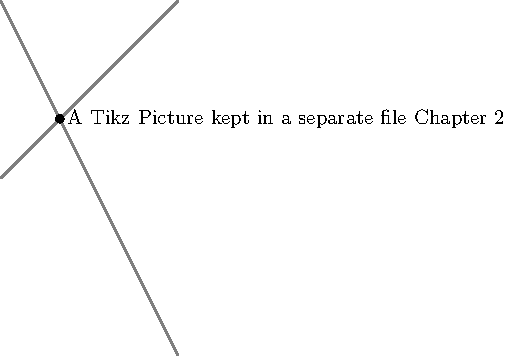
\includegraphics[alt={two lines intersecting at a point}]{Images/tikzPic.pdf}
  \caption{A Tikz figure with alt text and external reference}
\end{figure}

%Algorithm package can cause a parent key warning from tagpdf, but the actual
%tagging output is fine.
\begin{algorithm}
  \caption{Score Algorithm}
  \begin{algorithmic}[1]
    \State {\textbf{Input: }{$s$ is a sensor }}
    \Statex
    \For{$j\in \{1,2,\ldots,15\}$}
    \State Randomly choose $5$ days
    \For{$x\in \{1,2,\ldots,1000\}$}
    \parstate{Set $a$ to be something in this very long state that will have to be wrapped quite possibly around and around and around}
    \EndFor
    \EndFor
  \end{algorithmic}
\end{algorithm}

More text here. Now what is we ?

\printbibliography[heading=subbibnumbered]


\include{Body/ch6/ch6_future_and_conclusions}
\tagtool{flush-floats=subsection}% to keep floats where they are supposed to be in the tagging tree
\clearpage
\pagebreak
\end{document}

% IMPORTANT NOTES
% TABLE OF CONTENTS : First consider if the bib-no-break option above does what you want.
% TOPIC 1:  If you need a page break follow the steps below
% step1
% check before which chapter in the table of contents you want a page break
% step 2
% go the folder "body". There open the chapter tex file that you noted needed page break in the table of contents..
% step 3
% insert  \addtocontents{toc}{\protect\newpage} before the first line i.e. before the line \chapter{RESULTS}.

%%%%%%%%%%%%%%%%%%%%%%%%%%%%
% IN ORDER TO MAKE spacing changes in the title page got to the section in the isuthesis.cls file
% that starts with \long\def\maketitle{\begin{titlepage} and you can change the vskip/vspace amounts throughout

% use \caption{} for all captions of figures and tables, where the captions are not too long.

% Use \caption[]{} with the square brackets for short caption of figure or table that goes into the list of tables and list of figures, and the curly brackets can have long captions which go with the figure/ table.
